\section{Plugin Task}
\textbf{Choose a plugin (not explained in the lab sessions) that allows you to work with the volume model chosen by providing advanced tools tailored to specific tasks.}

The plugin or extension selected is the Airway segmentation. This is a simple module that segments the airway from a CT image. The user needs to specify the input volume and markup point placed in the trachea. The module automatically retrieves the convolution kernel of the image loaded from the DICOM.

To extract the segmentation view it has been done the next steps:
\begin{itemize}
    \item The first step is to select the CTChest volume data from the downloaded sample data.
    \item The seconde step is to create a point into a part of the airway volume that we want to segmentate. 
    To do it in the markup module we click a point list and select the part in any vision of the volume. 
    The point created is the F-1 that is placed into the trachea as it can be seen in the \textbf{\textit{\cref{fig:airway_point}}}.
    \begin{figure}[H]
        \centering
        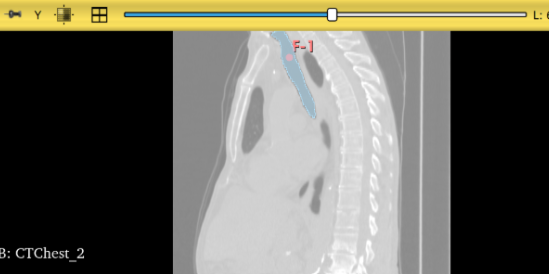
\includegraphics[width=0.7\textwidth]{img/ex61.png}
        \caption{Visualitzation of the vertical and lateral vision of the chest and the point F-1.}
        \label{fig:airway_point}
    \end{figure}
    \item Finally in the Airway segmentation module it is selected the CTChest volume and the point F-1 and it is applied to the segmentation. The F-1 point is clearly on the trachea of the patient since it is in the middle part of this vision of the chest. The air sections that can be seen in the \textbf{\textit{\cref{fig:airway_segmentation}}} correspond to the internal extreme parts of the right lung.
    \begin{figure}[H]
        \centering
        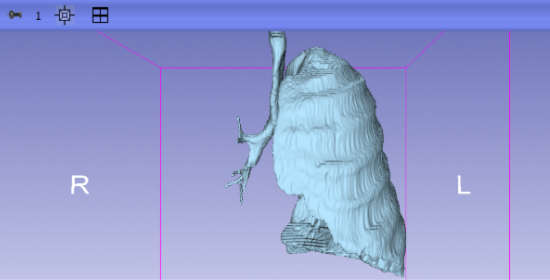
\includegraphics[width=0.7\textwidth]{img/ex62.png}
        \caption{Final result of the Airway Segmentation AI tool on the CTChest data based on the marker point used.}
        \label{fig:airway_segmentation}
    \end{figure}
\end{itemize}


In the \textbf{\textit{\cref{fig:airway_segmentation}}} can be observed as the result of the 
segmentation tool Airway Segmentation on the CTChest volume. It is clear how the 
segmentation tool shows the left lug but not the right. The correct side is clearly 
the right side because this segmentation extension was clearly to create images of 
air cavities as the trachea. The reason why this happens is because of a connection 
between the trachea and the left lung. The extension has a tool to determine the 
critical point of the trachea that connects to the lung - the bronchi - and uses 
it to differentiate the organs. For the right lung has properly worked since the 
terminations of the trachea that connects to the bronchi but for the left side it 
hasn’t worked properly since the lung appears in the figure as an airway conduct: 
the trachea. \\\\
% Add a name and a link to the plugin used
\textit{\textbf{\href{https://extensions.slicer.org/view/AirwaySegmentation/30822/win}{@KitwareMedical/slicer-extensions-webapp}}} \\
\textit{\textbf{\href{https://github.com/Slicer/SlicerAirwaySegmentation/commit/d3954e4}{Update README.md · Slicer/SlicerAirwaySegmentation@d3954e4 · GitHub}}}

